\newpage
\subsection{Pointing Pair / Triple}
Bei der Technik \textit{Pointing Pair / Triple} müssen, wie auch bei \textit{Hidden Single}, die Kandidatenlisten mehrerer Felder gleichzeitig betrachtet werden. Ausserdem ist diese Technik die erste, die Kandidaten aus Kandidatenlisten entfernt und nur bedingt zum Einsetzen von Zahlen in das Sudoku führt.\\
Es werden die Kandidatenlisten in Blöcken jeweils zeilen- und spaltenweise betrachtet. Die Technik \textit{Pointing Pair / Triple}
kann angewendet werden, wenn in einem Block ein Kandidat nur in Kandidatenlisten der selben Zeile oder Spalte vorkommt. Dann kann jedes weitere Vorkommen der Zahl in einer Kandidatenliste der selben Zeile oder Spalte entfernt werden. Das gilt, da die Zahl genau einmal in dem Block vorkommen muss. Da alle möglichen Vorkommen der Zahl in der selben Zeile oder Spalte liegen, ist klar, dass die Zahl in dieser Zeile oder Spalte vorkommt. Da sie kein zweites Mal in der Zeile oder Spalte vorkommen darf, muss sie aus allen Kandidatenlisten entfernt werden, die nicht im selben Block liegen.

\begin{figure}[h]
\begin{center}
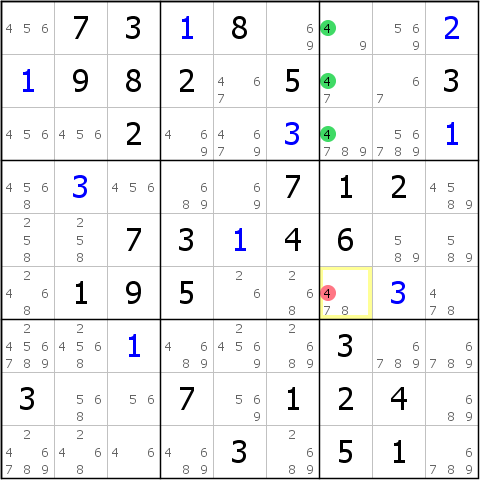
\includegraphics{./img/pointing_triple.png}
\caption{Pointing Triple}
\end{center}
\end{figure}

\noindent In \textbf{Abbildung 2.6} betrachten wir Block 3. Hier ist das Vorkommen der Zahl 4 in den Kandidatenlisten auf Spalte 7 beschränkt. Wie oben beschrieben, können nun alle weiteren Vorkommen in der selben Spalte, die nicht in Block 3 liegen aus den Kandidatenlisten entfernt werden. Diese sind in der Abbildung rot markiert. Das führt nicht dazu, dass eine neue Zahl in das Sudoku eingetragen wird. Dennoch ist das Sudoku nun genauer bestimmt, da weniger Möglichkeiten übrig sind.